% Afficher des recommendations concernant la syntaxe.
\RequirePackage[orthodox,l2tabu]{nag}
\RequirePackage{luatex85}
% Paramètres du document.
\documentclass[%
a5paper%                       Taille de page.
,11pt%                         Taille de police.
,DIV=auto%                       Plus grand => des marges plus petites.
,titlepage=on%                 Faut-il une page de titre ?
,headings=optiontoheadandtoc%  Effet des paramètres optionnels de section.
,headings=small%
,parskip=false%
,openany%
]{scrbook}
\renewcommand*\partheademptypage{\thispagestyle{empty}}
\def\staffsize{0}%%%%% Taille des partitions ly
\newcounter{facteur}\setcounter{facteur}{17}%%%%%%%%%%%%%% Paramètre pour la taille globale des partitions. par défaut~: 17
%\usepackage{geometry}
\usepackage{gredoc,mudoc,lyluatex}
\usepackage{pdfpages,transparent,array,ltablex}

%%%%%%%%%%%%%%%%%%%%%%% Paramètres variables %%%%%%%%%%%%%%%%%%%%%%%%%%%%%%%%%%%%%%%%%%%%%%%%%%
%%% Taille des partitions grégoriennes.                                                      %%
%\grechangedim{overhepisemalowshift}{.7mm}{scalable}
%\grechangedim{hepisemamiddleshift}{1.4mm}{scalable}
%\grechangedim{overhepisemahighshift}{2.1mm}{scalable}
%\grechangedim{vepisemahighshift}{2.1mm}{scalable}
%\grechangestafflinethickness{50} %%% epaisseur des lignes
\grechangestaffsize{\value{facteur}}%%%%% 
%%%%%%%%%%%%%%%%%%%%%%%%%%%%%%%%%%%%%%%%%%%%%%%%%%%%%%%%%%%%%%%%%%%%%%%%%%%%%%%%%%%%%%%%%%%%%%%
% Par souci de clarté, la définition des commandes est reportée dans un document annexe.

%\addtolength{\voffset}{2mm}\addtolength{\headsep}{-2mm}
%\setlength{\extrarowheight}{2mm}

\addto\captionsfrench{%
  \renewcommand{\indexname}{Index des chants}%
}

\pdfcompresslevel=9

\newcommand{\lieu}[1]{\hfill\linebreak[3]\hspace*{\stretch{1}}\nolinebreak\mbox{\emph{(#1)}}}


\newcommand{\schola}[1]{}\newcommand{\foule}[1]{#1}
\providecommand{\dest}{foule}
\newcommand{\imagecentre}[2]{
\begin{center} \includegraphics[height=#1]{img/#2} \end{center}}

%\newcommand{\bgimage}[1]{%
%\raisebox{-.45\paperheight}[0pt][0pt]{%
%  \transparent{0.3}%
%  \includegraphics[width=.7\paperwidth,height=.7\paperheight,keepaspectratio=true]{img/#1}%
%  }%
%}

\def\arraystretch{1.2}

\newcommand{\reponsegras}[2]{
\versio{\textbf{#1}}{{#2}}}

\newcommand{\ligne}[2]{
\begin{center}
\greseparator{#1}{#2}
\end{center}}

\title{Livret du Pèlerin de Fontpeyrine}
\date{\includegraphics[width=.3\textwidth]{img/Fontpeyrine-Vierge-source.png}}

\let\oldaddchap\addchap
\def\addchap#1{\oldaddchap{#1}\markright{Livret du Pèlerin de Fontpeyrine}}

\def\blindsection#1{\markright{#1}\addcontentsline{toc}{section}{#1}}
%%%%%%%%%%%%%%%%%%%%%%%%%%%%%%%%%%%%%%%%%%%%%%%%%%%%%%%%%%%%%%%%%%%%%%%%%%%%%%%%
%%%%%%%%%%%%%%%%%%%%%% Début du document %%%%%%%%%%%%%%%%%%%%%%%%%%%%%%%%%%%%%%%
%%%%%%%%%%%%%%%%%%%%%%%%%%%%%%%%%%%%%%%%%%%%%%%%%%%%%%%%%%%%%%%%%%%%%%%%%%%%%%%%
\begin{document}
\maketitle

\addchap{Prière à Notre-Dame de Fontpeyrine}
{\centering {\textit{\Large{Notre-Dame de Fontpeyrine,\vfill
qui depuis des siècles accordez de nombreuses faveurs\vfill
à ceux qui ont recours à votre puissante intercession,\vfill
obtenez, nous vous en supplions,\vfill
à nous vos humbles serviteurs, \vfill
en souvenir de votre bienheureuse Nativité,\vfill
ce complément de grâce\vfill
que nous implorons à genoux devant vous.\vfill
Nous l’attendons avec confiance,\vfill
malgré notre indignité, ô Mère du Sauveur,\vfill
de votre maternelle bonté\vfill
et de votre bienveillante protection.\vfill
Ainsi soit-il.\vfill
Notre-Dame de Fontpeyrine, priez pour nous (trois fois).}}}}
\clearpage

\addchap{Cantiques}
%\blindsection{Cantiques}
\section{Vierge de Fontpeyrine}
\lilypondfile[staffsize=15]{ly/ViergeDeFontpeyrine/ViergeDeFontpeyrine.ly}
\chanson[position=2col,numero=2,premiercouplet=2,refrain=non]{ly/ViergeDeFontpeyrine/ViergeDeFontpeyrine}
%\lilypondfile[staffsize=15]{ly/ViergeDeFontpeyrine/ViergeDeFontpeyrine-dernier.ly}

\clearpage

\needspace{8\baselineskip}
\section{C'est le Périgord}
\lilypondfile[staffsize=15]{ly/CestLePerigord/CestLePerigord.ly}
\chanson[position=2col,numero=2,premiercouplet=2,refrain=non]{ly/CestLePerigord/CestLePerigord}

\needspace{8\baselineskip}
\section{Notre-Dame du Périgord}
\lilypondfile[staffsize=15]{ly/NotreDameDuPerigord/NotreDameDuPerigord.ly}
\chanson[numero=2,premiercouplet=2,refrain=non]{ly/NotreDameDuPerigord/NotreDameDuPerigord}

\needspace{8\baselineskip}
\section{Les saints et les anges}
\chanson[position=2col,numero=1]{ly/AveMariaDeLourdes/LesSaintsEtLesAnges}


\needspace{8\baselineskip}
\section{J'irai la voir un jour}
\chanson[position=2col,numero=1]{ly/JIraiLaVoirUnJour/JIraiLaVoirUnJour}

\needspace{8\baselineskip}
\section{Vierge sainte}
\chanson[position=2col,numero=1]{ly/ViergeSainte/ViergeSainte}

\needspace{8\baselineskip}
\section{Laudate Mariam}
\chanson[position=2col,numero=1]{ly/LaudateMariam/LaudateMariam}

\needspace{8\baselineskip}
\section{Ave Maris Stella}
\chanson[position=2col,numero=1]{ly/AveMarisStella/AveMarisStella}

\needspace{15\baselineskip}
\section{Reine de France}
\chanson[numero=1]{ly/ReineDeFrance/ReineDeFrance}

\needspace{8\baselineskip}
\section{Je mets ma confiance}
\chanson[position=2col,numero=1]{ly/JeMetsMaConfiance/JeMetsMaConfiance}

\needspace{8\baselineskip}
\section{Chez nous, soyez Reine}
\chanson[position=2col,numero=1]{ly/ChezNousSoyezReine/ChezNousSoyezReine}

\needspace{8\baselineskip}
\section{Tandis que le monde proclame}
\chanson[position=2col,numero=1]{ly/ParleCommandeRegne/ParleCommandeRegne}

\needspace{8\baselineskip}
\section{Je suis chrétien}
\chanson[position=2col,numero=1]{ly/JeSuisChretien/JeSuisChretien}

\needspace{8\baselineskip}
\section{Nous voulons Dieu}
\chanson[position=2col,numero=1]{ly/NousVoulonsDieu/NousVoulonsDieu}

\needspace{8\baselineskip}
\section{Litanies de la très sainte Vierge}
\begin{litaniae}
\invocatio{Kýrie, eléison.}{Seigneur, ayez pitié de nous.}
\invocatio{Christe, eléison.}{Jésus-Christ, ayez pitié de nous.}
\invocatio{Kýrie, eléison.}{Seigneur, ayez pitié de nous.}
\invocatio{Christe, audi nos.}{Jésus-Christ, écoutez-nous.}
\invocatio{Christe, exáudi nos.}{Jésus-Christ, exaucez-nous.}
\rinvocatio{Pater de cælis, Deus,}{Père céleste qui êtes Dieu,}{miserére nobis.}{ayez pitié de nous.}
\invocatio{Fili, Redémptor mundi, Deus,}{Fils Rédempteur du monde, qui êtes Dieu,}
\invocatio{Spíritus Sancte, Deus,}{Esprit Saint, qui êtes Dieu,}
\invocatio{Sancta Trínitas, unus Deus,}{Trinité Sainte, qui êtes un seul Dieu,}
\rinvocatio{Sancta María}{Sainte Marie}{ora pro nobis.}{priez pour nous.}
\invocatio{Sancta Dei Genitrix,}{Sainte Mère de Dieu,}
\invocatio{Sancta Virgo virginum,}{Sainte Vierge des vierges,}
\invocatio{Mater Christi,}{Mère du Christ,}
\invocatio{Mater Ecclesiae,}{Mère de la Sainte Eglise,}
\invocatio{Mater divinae gratiae,}{Mère de la divine grâce,}
\invocatio{Mater purissima,}{Mère très pure,}
\invocatio{Mater castissima,}{Mère très chaste,}
\invocatio{Mater inviolata,}{Mère toujours Vierge,}
\invocatio{Mater intemerata,}{Mère sans tache,}
\invocatio{Mater amabilis,}{Mère aimable,}
\invocatio{Mater admirabilis,}{Mère admirable,}
\invocatio{Mater boni consilii,}{Mère du bon conseil,}
\invocatio{Mater Creatoris,}{Mère du Créateur,}
\invocatio{Mater Salvatoris,}{Mère du Sauveur,}
\invocatio{Virgo prudentissima,}{Vierge très prudente,}
\invocatio{Virgo veneranda,}{Vierge vénérable,}
\invocatio{Virgo praedicanda,}{Vierge digne de louange,}
\invocatio{Virgo potens,}{Vierge puissante,}
\invocatio{Virgo clemens,}{Vierge clémente,}
\invocatio{Virgo fidelis,}{Vierge fidèle,}
\invocatio{Speculum justitiae,}{Miroir de justice,}
\invocatio{Sedes sapientiae,}{Trône de la sagesse,}
\invocatio{Causa nostrae laetiae,}{Cause de notre joie,}
\invocatio{Vas spirituale,}{Vase spirituel,}
\invocatio{Vas honorabile,}{Vase d'honneur,}
\invocatio{Vas insigne devotionis,}{Vase insigne de dévotion,}
\invocatio{Rosa mystica,}{Rose mystique,}
\invocatio{Turris Davidica,}{Tour de David,}
\invocatio{Turris ebumea,}{Tour d'ivoire,}
\invocatio{Domus aurea,}{Maison d'or,}
\invocatio{Fœderis arca,}{Arche d'alliance,}
\invocatio{Janua Caeli,}{Porte du ciel,}
\invocatio{Stella matutina,}{Étoile du matin,}
\invocatio{Salus infirmorum,}{Salut des infirmes,}
\invocatio{Refugium peccatorum,}{Refuge des pécheurs,}
\invocatio{Consolatrix afflictonim,}{Consolatrice des affligés,}
\invocatio{Auxilium Christianorum,}{Secours des chrétiens,}
\invocatio{Regina Angelorum,}{Reine des Anges,}
\invocatio{Regina Patriarcharum,}{Reine des Patriarches,}
\invocatio{Regina Prophetarum,}{Reine des Prophètes.}
\invocatio{Regina Apostolorum,}{Reine des Apôtres,}
\invocatio{Regina Martyrum,}{Reine des Martyrs,}
\invocatio{Regina Confessorum,}{Reine des Confesseurs,}
\invocatio{Regina Virginum,}{Reine des Vierges,}
\invocatio{Regina Sanctorum omnium,}{Reine de tous les Saints}
\invocatio{Regina sine labe originali concepta}{Reine conçue sans le péché originel,}
\invocatio{Regina in caelum assumpta,}{Reine élevée aux Cieux,}
\invocatio{Regina sacratissimi Rosarii,}{Reine du très saint Rosaire,}
\invocatio{Regina pacis,}{Reine de la paix,}
\rinvocatio{Agnus Dei, qui tollis peccáta mundi,}{Agneau de Dieu, qui effacez les péchés du monde,}%
{parce nobis, Dómine.}{pardonnez-nous, Seigneur.}
\rinvocatio{Agnus Dei, qui tollis peccáta mundi,}{Agneau de Dieu, qui effacez les péchés du monde,}%
{exáudi nos, Dómine.}{exaucez-nous, Seigneur.}
\rinvocatio{Agnus Dei, qui tollis peccáta mundi,}{Agneau de Dieu, qui effacez les péchés du monde,}%
{miserére nobis.}{ayez pitié de nous.}
\end{litaniae}
\versio{\vb. Ora pro nobis, sancta Dei Génetrix,}{Priez pour nous sainte Mère de Dieu}
\versio{\rb. Ut digni efficiámur promissiónibus Christi.}{Afin que nous soyons dignes des promesses du Christ}
\versio{\centering{Orémus}

Concéde nos fámulos tuos, quǽsumus, Dómine Deus, perpétua mentis et córporis sanitáte gaudére : et, gloriósa beátæ Maríæ semper Vírginis intercessióne, a præsénti liberári tristítia et ætérna pérfrui lætítia. Per Dóminum.}
{\centering{Prions.}

Seigneur, daignez nous accorder, à nous vos serviteurs, de jouir toujours de la santé de l'âme et du corps; et par la glorieuse intercession de la bienheureuse Marie toujours Vierge, délivrez-nous des tristesses de la vie présente, et donnez-nous d'avoir part aux joies éternelles. Par Jésus-Christ Notre Seigneur.}

%%%%%%%%%%%%%%%%%%%%%%%%%%%%%%%%%%%%%%%%%%%%%%%%%%%%%%%%%%%%%%%%%%%%%%%%%%%%%%%%
\subsection*{Introït}
\rubrica{Pendant que le l'officiant se prépare à monter à l'autel avec les \emph{prières au bas de l'autel}, nous chantons l'Introït (voir à la messe du jour).}

\rubrica{On chante ensuite le \emph{Kyrie} et le \emph{Gloria}}

\subsection*{Oraison Collecte}
\rubrica{Cette oraison est appelée \emph{Collecte} parce que le prêtre y réunit, pour les offrir à Dieu, les prières et les vœux des fidèles assemblés. Elle termine généralement ainsi : «~Par Jésus-Christ Notre-Seigneur », pour nous montrer que nous ne pouvons aller au Père que par son divin Fils.
\rubrica{Voir l'oraison à la messe du jour}

\subsection*{Épître}
\rubrica{Voir à la messe du jour. A la fin de l'épître, on répond~:}
\textbf{\rb\ Deo grátias.}

\susection*{Graduel et Alléluia}
\rubrica{Graduel, Alléluia sont des chants de méditation sur les lectures ou le mystère liturgique de ce jour. \emph{Alleluia} signifie "louez Dieu". L'Alléluia se prolonge dans une mélodie ornée qui exprime la joie spirituelle au-delà des paroles.}
\rubrica{Voir à la messe du jour}

\subsection*{Évangile.}
\rubrica{On chante le saint Évangile tourné vers le Nord (le chœur étant normalement orienté vers l'Est) parce que le Nord symbolise les âmes qui se trouvent dans la froideur de l'infidélité et de l'ignorance du Christ, et qui sont éveillées par le souffle du Saint-Esprit.}
\rubrica{Voir à la messe du jour. A la fin de l'évangile, on répond~:}
\reponsegras{%
\rb\ Laus tibi Christe.}{%
\rb\ Christ, louange à vous.}

\subsection*{Offertoire}
\rubrica{À l'Offertoire l'Église offre le Corps et le Sang du Christ, représentés par le pain et le vin. Notre Seigneur a communiqué à son Église le pouvoir d'offrir le même sacrifice qu'il offrit sur la Croix. L'Église s'y unit comme victime. Nous sommes donc une seule victime avec le Christ, unissant nos propres offrandes et nos sacrifices à celui du Christ et de l'Église. Notre participation à cette offrande est exprimée par le chant de l'offertoire.}
Recevez, Père saint, Dieu éternel et tout-puissant, cette offrande sans tache, que moi, votre indigne serviteur, je vous présente, à vous, mon Dieu vivant et vrai, pour mes péchés, offenses et négligences sans nombre, pour tous ceux qui m'entourent, ainsi que pour tous les fidèles vivants et morts~: qu'elle serve à mon salut et au leur pour la vie éternelle. Ainsi soit-il.

Nous vous offrons, Seigneur, le calice du salut, et nous demandons à votre clémence qu'il s'élève en parfum agréable devant votre divine Majesté, pour notre salut et celui du monde entier. \mbox{Ainsi soit-il}.\looseness=1

\versio{%
Oráte, fratres : ut meum ac vestrum sacrifícium acceptábile fiat apud Deum Patrem omnipoténtem.}{%
Priez, mes frères, pour que mon sacrifice, qui est aussi le vôtre, puisse être agréé par Dieu le Père tout-puissant.}

\rubrica{À la messe lue on répond :}

\versio{%
℟. Suscípiat Dóminus sacrifícium de mánibus tuis, ad laudem et glóriam nóminis sui, ad utilitátem quoque nostram, totiúsque Ecclésiæ suæ sanctæ.}{%
℟. Que le Seigneur reçoive de vos mains le sacrifice, à la louange et à la gloire de son Nom, ainsi que pour notre bien et celui de toute sa sainte Église.}
\subsection*{%
Oraison Secrète%
}

\rubrica{Voir à la messe du jour.}

\subsection*{Oblation du Sacrifice}

\rubrica{Commence ici la partie la plus sacrée de la Liturgie : le sacrifice réel et sacramentel où le prêtre immole le Christ. \emph{Vraiment à cette heure très redoutable il faut tenir haut son cœur vers Dieu, et non en bas vers la terre et les affaires terrestres. D'autorité donc le pontife  enjoint à cette heure à tous de laisser de côté les soucis, les sollicitudes domestiques, et de tenir leur cœur au ciel vers Dieu ami des hommes.} \mbox{(S. Cyrille de Jérusalem)}}

\subsection*
\rubrica{Par le chant de la Préface le prêtre rend grâces à Dieu au nom de l'Église pour l'œuvre du salut réalisée par Jésus-Christ.}
\subsection*{%
Sanctus%
}

\rubrica{L'hymne au Dieu trois fois saint se compose d'une vision du prophète Isaïe (Is. 6,3) et des acclamations chantées lors de l'entrée triomphale du Christ à Jérusalem.}

\subsection*{Consécration}
\rubrica{Le prêtre récite alors l'histoire de l'institution de l'Eucharistie en accomplissant les mêmes gestes que le Christ.}

\versio{%
Qui prídie quam paterétur, accépit panem in sanctas ac venerábiles manus suas, et elevátis óculis in cælum ad te Deum Patrem suum omnipoténtem, tibi grátias agens, bene ✠ díxit, fregit, dedítque discípulis suis, dicens~: Accípite, et manducáte ex hoc omnes.}{%
Celui-ci, la veille de sa Passion, prit du pain dans ses mains saintes et adorables, et, les yeux levés au ciel vers vous, Dieu, son Père tout-puissant, vous rendant grâces, il ✠ bénit ce pain, le rompit et le donna à ses disciples en disant~: Prenez et mangez-en tous.}


\rubrica{Le prêtre prononce alors les paroles mêmes de Notre-Seigneur. Par ces paroles il opère la conversion du pain au saint Corps du Christ.}

\versio{%
\scalebox{.91}[1]{\textsc{\addfontfeatures{Renderer=Basic}Hoc est enim Corpus meum.}}\par%
}{%
\textsc{\addfontfeatures{Renderer=Basic}Car ceci est mon Corps.}\par%
}

%\vspace{1\baselineskip plus 2\baselineskip}

\rubrica{Ces paroles étant prononcées, le prêtre fait la génuflexion pour adorer le saint Corps, l'élève pour le présenter à l'adoration des fidèles, puis reprend le récit de l'institution de l'eucharistie~:}

\versio{%
Símili modo postquam cenátum est, accípiens et hunc præclárum Cálicem in sanctas ac venerábiles manus suas~: item tibi grátias agens, bene ✠ díxit, dedítque discípulis suis, dicens~: Accípite, et bíbite ex eo omnes.}{%
De même, après le repas, il prit aussi ce précieux calice dans ses mains saintes et adorables, vous rendit grâces encore, le ✠ bénit et le donna à ses disciples en disant~: Prenez et buvez-en tous.}

\rubrica{Prononçant alors les paroles mêmes de Notre-Seigneur, le prêtre opère la conversion du vin au précieux Sang du Christ.}
%
\nopagebreak\smallskip%
%
\versio{%
\textsc{\addfontfeatures{Renderer=Basic}Hic est enim Calix Sánguinis mei, novi et ætérni Testaménti~: mystérium fídei~: qui pro vobis et pro multis effundétur in remissiónem peccatórum.}%
}{%
\textsc{\addfontfeatures{Renderer=Basic}Car ceci est le Calice de mon Sang, le Sang de l'Alliance nouvelle et éternelle, le mystère de la foi, qui sera versé pour vous et pour un grand nombre en rémission des péchés.}%
}

\smallskip

\versio{%
Hæc quotiescúmque fecéritis, in mei memóriam faciétis.}{%
Toutes les fois que vous ferez cela, vous le ferez en mémoire de moi.}%

%\vspace{1\baselineskip plus 2\baselineskip}

\rubrica{Ces paroles étant prononcées, le prêtre fait la génuflexion pour adorer le précieux Sang. Il l'élève pour le présenter à l'adoration, et fait de nouveau la génuflexion.}

\subsection*{Communion}
\subsection*{%
Agnus Dei%
}

\rubrica{Les Hébreux immolaient un agneau en mémoire de leur délivrance de la captivité d'Égypte. Cet agneau était la figure du véritable Agneau immolé pour nous délivrer de la captivité du péché et du démon. Selon les paroles de S.~Jean-Baptiste, il est l'\emph{Agneau de Dieu qui enlève le péché du monde.}}

\versio{%
Agnus Dei, qui tollis peccáta mundi, miserére nobis. \emph{bis}%
}{%
Agneau de Dieu, qui ôtez les péchés du monde, ayez pitié de nous. \emph{bis}%
}%

\versio{%
Agnus Dei, qui tollis peccáta mundi, dona nobis pacem.%
}{%
Agneau de Dieu, qui ôtez les péchés du monde, donez-nous la paix.%
}%

Seigneur Jésus-Christ, qui avez dit à vos Apôtres~: C'est la paix que je vous laisse en héritage, c'est ma paix je vous donne, ne regardez pas mes péchés, mais la foi de votre Église~; daignez, selon votre volonté, lui donner la paix et la rassembler dans l'unité, vous qui, étant Dieu, vivez et régnez dans tous les siècles des siècles. Ainsi soit-il.
\rubrica{Le baiser de paix, manifestant l'union dans la paix du Christ, est hiérarchiquement transmis de l'autel jusqu'au dernier degré du clergé. \emph{Ne pense pas que ce baiser soit comme ceux qui se donnent sur la place entre amis ordinaires. Il unit les âmes entre elles~; il est réconciliation, et pour cette raison il est saint.} (S.~Cyrille de Jérusalem)}
Seigneur Jésus-Christ, Fils du Dieu vivant, qui, accomplissant la volonté du Père dans une œuvre commune avec le Saint-Esprit, avez par votre mort donné la vie au monde, délivrez-moi par votre Corps et votre Sang infiniment saints de tous mes péchés et de tout mal. Faites que je reste toujours attaché à vos commandements, et ne permettez pas que je sois jamais séparé de vous, qui, étant Dieu, vivez et régnez avec Dieu le Père et le Saint-Esprit dans les siècles des siècles. Ainsi soit-il.
Seigneur Jésus-Christ, si j'ose recevoir votre Corps malgré mon indignité, que cela n'entraîne pour moi ni jugement ni condamnation, mais, par votre miséricorde, me serve de sauvegarde et de remède pour l'âme et pour le corps, vous qui, étant Dieu, vivez et régnez avec Dieu le Père en l'unité du Saint-Esprit, dans tous les siècles des siècles. Ainsi soit-il.

\rubrica{Après avoir communié, le prêtre se retourne vers les fidèles en leur présentant le saint Corps du Christ.}

\versio{%
Ecce Agnus Dei, ecce qui tollis peccáta mundi.}{%
Voici l'Agneau de Dieu, voici celui qui enlève les péchés du monde.}

\rubrica{Nous répondons par les paroles du bienheureux centurion. Cette fois ce n'est plus la guérison d'un serviteur que nous demandons, mais celle de notre âme.}
%
\versio{%
Dómine, non sum dignus, ut intres sub tectum meum~: sed tantum dic verbo, et sanábitur ánima mea. \emph{ter}}{%
Seigneur, je ne suis pas digne que vous entriez sous mon toit~; mais dites seulement une parole, et mon âme sera guérie. \emph{ter}}

\rubrica{Aux premiers siècles le diacre invitait ceux qui ne pouvaient pas communier à se retirer. Aujourd'hui l'Église est plus indulgente mais les conditions pour communier sont les mêmes~: \textbf{être baptisé et catholique~; ne pas avoir de péché mortel sur la conscience, ce qui suppose notamment l'observation des lois de l'Église au sujet du mariage~; avoir observé le jeûne eucharistique.} La discipline actuelle est d'une heure de jeûne avant la communion. Nous conseillons cependant de s'en tenir à la discipline d'avant le Concile Vatican II~: trois heures pour la nourriture solide, une heure pour le liquide non alcoolisé.\\
La sainte communion est reçue à genoux et directement dans la bouche.}

\needspace{3\baselineskip}
\rubrica{En donnant la sainte Eucharistie, le prêtre dit~:}

\versio{%
Corpus Dómini nostri Iesu Christi custódiat ánimam tuam in vitam ætérnam. Amen.}{%
Que le Corps de Notre Seigneur Jésus-Christ garde votre âme pour la vie éternelle. Ainsi soit-il.}

\rubrica{%
On ne répond rien.}

\rubrica{%
Jésus-Christ est le Bon Pasteur qui donne sa vie pour ses brebis. \emph{Je suis venu pour qu'ils aient la vie et qu'ils l'aient en abondance}. Il nous communique cette vie dans la sainte Eucharistie.%
}

\subsection*{Chant de communion et Postcommunion}
\rubrica{Voir à la messe du jour}
%%%%%%%%%%%%%%%%%%%%%%%%%%%%%%%%%%%%%%%%%%%%%%%%%%%%%%%%%%%%%%%%%%%%%%%%%%%%%%%%
%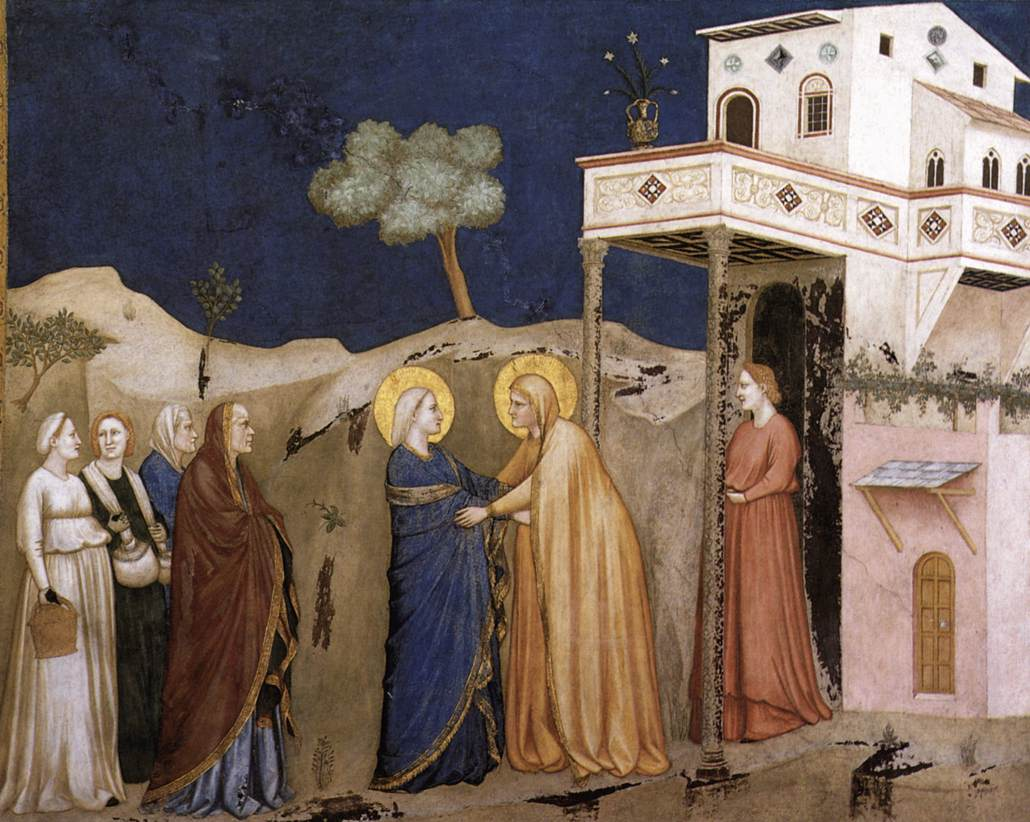
\includegraphics[width=\textwidth]{img/VisitationGiotto.jpg}

\addchap{Messe de la Visitation - 2 juillet}

\rubrica{ Le 2 juillet 1769, fête de la Visitation, un orage, tel qu'on n'en avait pas vu depuis longtemps, dévasta les campagnes de Saint-Cyprien, du Bugue, et de Terrasson. La paroisse de Tursac et le sanctuaire de Fontpeyrine furent seuls épargnés.
C'est pourquoi, les représentants de la ville de Tursac et sa pieuse population firent vœu d'aller au sanctuaire tous les ans en procession, au jour anniversaire du bienfait, pour remercier Notre-Dame de Fontpeyrine.}

\rubrica{La messe est à la page \emph{\pageref{Ordo}}, excepté les textes propres qui suivent~:}

\begin{multicols}{2}
\subsection*{Introït}
{Salut, ô Mère sainte~; mère qui avez enfanté le Roi qui régit le ciel et la terre dans les siècles des siècles.}
De mon cœur a jailli une parole excellente, c’est que je consacre mes œuvres à mon Roi. \vb\ Gloire au Père.

\subsection*{Collecte}
{Prions\\
Seigneur, nous vous prions d’accorder à vos serviteurs le don de la grâce céleste~: et, comme l’enfantement de la bienheureuse Vierge a été le principe de leur salut~; qu’ainsi la pieuse solennité de sa Visitation leur procure un accroissement de paix. Par Notre Seigneur.}
{\textbf{ \rb\ Amen.}}


\subsection*{Épître : Lecture du Livre de la Sagesse}
\rubrica{Cant. 2, 8-14.}
Voici qu’il vient, bondissant sur les montagnes, sautant sur les collines. Mon bien-aimé est semblable à la gazelle, ou au faon des biches. Le voici, il est derrière notre mur, regardant par la fenêtre, épiant par le treillis. Voici, mon bien-aimé me dit~: "Lève-toi, hâte-toi, mon amie, ma colombe, ma belle, et viens ! Car voici que l’hiver est fini~; la pluie a cessé, elle a disparu. Les fleurs ont paru sur notre terre, le temps des chants est arrivé~; la voix de la tourterelle s’est fait entendre dans nos campagnes~; le figuier pousse ses fruits naissants, les vignes en fleur donnent son parfum. Lève-toi, mon amie, ma belle, et viens ! Ma colombe, qui te tiens dans la fente du rocher, dans l’abri des parois escarpées, montre-moi ton visage, que ta voix résonne à mes oreilles~; car ta voix est douce, et ton visage charmant.
\textbf{\rb\ Deo grátias.}

\subsection*{Antiennes}
Vous êtes bénie et digne de vénération, Vierge Marie, qui avez été mère du Sauveur, sans que votre pureté ait subi d’atteinte. Vierge, Mère de Dieu, celui que tout l’univers ne peut contenir, s’est enfermé dans votre sein en se faisant homme.

Alléluia, alléluia. \vb\ Vous êtes heureuse, sainte Vierge Marie, et tout à fait digne de louange, car de vous est sorti le soleil de justice, le Christ notre Dieu. Alléluia.

\subsection*{Lecture du saint Évangile selon saint Luc.}
\rubrica{Luc 1, 39-47.}
En ces jours-là, Marie partit et s’en alla en hâte vers la montagne, en une ville de Juda. Et elle entra dans la maison de Zacharie, et salua Élisabeth. Or, quand Élisabeth entendit la salutation de Marie, l’enfant tressaillit dans son sein, et elle fut remplie du Saint-Esprit. Et elle s’écria à haute voix, disant~: "Vous êtes bénie entre les femmes, et le fruit de vos entrailles est béni. Et d’où m’est-il donné que la mère de mon Seigneur vienne à moi ? Car votre voix, lorsque vous m’avez saluée, n’a pas plus tôt frappé mes oreilles, que l’enfant a tressailli de joie dans mon sein. Heureuse celle qui a cru ! Car elles seront accomplies les choses qui lui ont été dites de la part du Seigneur !" Et Marie dit~: "Mon âme glorifie le Seigneur, et mon esprit tressaille de joie en Dieu, mon Sauveur".
{\textbf {\rb\ Laus tibi Christe.}}

\rubrica{Chant du Credo page \pageref{Credo}}

\subsection*{Antienne d'Offertoire}
Vous êtes bienheureuse, Vierge Marie, qui avez porté le Créateur de toutes choses ; vous avez enfanté celui qui vous a créée, et vous demeurez à jamais Vierge.

\subsection*{Oraison Secrète}
Qu’elle nous porte secours, Seigneur, la bonté de votre Fils unique, qui né d’une Vierge, n’a point altéré l’intégrité de sa Mère mais l’a consacrée, afin que nous purifiant de nos fautes en la solennité de sa Visitation, il vous rende notre oblation agréable, lui Jésus-Christ notre Seigneur.

\subsection*{Chant de communion}
Bienheureux le sein de la Vierge Marie, qui a porté le Fils du Père éternel.

\needspace{3\baselineskip}
\subsection*{Postcommunion}
{Nous avons reçu, Seigneur, les choses saintes qui vous sont offertes en cette solennité annuelle, faites, nous vous en supplions, qu’elles nous donnent les remèdes spirituels utiles à la vie temporelle et conduisant à la vie éternelle.}
\textbf{ \rb\ Amen.}

\end{multicols}

\addchap{Messe de l'Assomption - 15 août}

%\rubrica{ Le 2 juillet 1769, fête de la Visitation, un orage, tel qu'on n'en avait pas vu depuis longtemps, dévasta les campagnes de Saint-Cyprien, du Bugue, et de Terrasson. La paroisse de Tursac et le sanctuaire de Fontpeyrine furent seuls épargnés. C'est pourquoi, les représentants de la ville de Tursac et sa pieuse population firent vœu d'aller au sanctuaire tous les ans en procession, au jour anniversaire du bienfait, pour remercier Notre-Dame de Fontpeyrine.}

\rubrica{La messe est à la page \emph{\pageref{Ordo}} excepté les textes propres qui suivent~:}

\begin{multicols}{2}
\subsection*{Introït}
{Salut, ô Mère sainte~; mère qui avez enfanté le Roi qui régit le ciel et la terre dans les siècles des siècles.}
De mon cœur a jailli une parole excellente, c’est que je consacre mes œuvres à mon Roi. \vb\ Gloire au Père.

\subsection*{Collecte}
{Prions\\
Seigneur, nous vous prions d’accorder à vos serviteurs le don de la grâce céleste~: et, comme l’enfantement de la bienheureuse Vierge a été le principe de leur salut~; qu’ainsi la pieuse solennité de sa Visitation leur procure un accroissement de paix. Par Notre Seigneur.}
{\textbf \rb\ Amen.}

\subsection*{Antiennes}
Vous êtes bénie et digne de vénération, Vierge Marie, qui avez été mère du Sauveur, sans que votre pureté ait subi d’atteinte. Vierge, Mère de Dieu, Celui que tout l’univers ne peut contenir, s’est enfermé dans votre sein en se faisant homme.

Alléluia, alléluia. \vb\ Vous êtes heureuse, sainte Vierge Marie, et tout à fait digne de louange, car de vous est sorti le soleil de justice, le Christ notre Dieu. Alléluia.

\subsection*{Epître : Lecture du Livre de la Sagesse.}
\rubrica{Cant. 2, 8-14.}
Voici qu’il vient, bondissant sur les montagnes, sautant sur les collines. Mon bien-aimé est semblable à la gazelle, ou au faon des biches. Le voici, il est derrière notre mur, regardant par la fenêtre, épiant par le treillis. Voici, mon bien-aimé me dit~: "Lève-toi, hâte-toi, mon amie, ma colombe, ma belle, et viens ! Car voici que l’hiver est fini~; la pluie a cessé, elle a disparu. Les fleurs ont paru sur notre terre, le temps des chants est arrivé~; la voix de la tourterelle s’est fait entendre dans nos campagnes~; le figuier pousse ses fruits naissants, les vignes en fleur donnent son parfum. Lève-toi, mon amie, ma belle, et viens ! Ma colombe, qui te tiens dans la fente du rocher, dans l’abri des parois escarpées, montre-moi ton visage, que ta voix résonne à mes oreilles~; car ta voix est douce, et ton visage charmant.
\textbf{\rb\ Deo grátias.}

\subsection*{Lecture du Saint Évangile selon saint Luc.}
\rubrica{Luc. 1, 39-47.}
En ces jours-là~: Marie partit et s’en alla en hâte vers la montagne, en une ville de Juda. Et elle entra dans la maison de Zacharie, et salua Élisabeth. Or, quand Élisabeth entendit la salutation de Marie, l’enfant tressaillit dans son sein, et elle fut remplie du Saint-Esprit. Et elle s’écria à haute voix, disant~: "Vous êtes bénie entre les femmes, et le fruit de vos entrailles est béni. Et d’où m’est-il donné que la mère de mon Seigneur vienne à moi ? Car votre voix, lorsque vous m’avez saluée, n’a pas plus tôt frappé mes oreilles, que l’enfant a tressailli de joie dans mon sein. Heureuse celle qui a cru ! Car elles seront accomplies les choses qui lui ont été dites de la part du Seigneur !" Et Marie dit~: "Mon âme glorifie le Seigneur, et mon esprit tressaille de joie en Dieu, mon Sauveur".
{\textbf \rb\ Laus tibi Christe.}

\subsection*{Antienne d'offertoire}
Vous êtes bienheureuse, Vierge Marie, qui avez porté le Créateur de toutes choses ; vous avez enfanté celui qui vous a créée, et vous demeurez à jamais Vierge.

\subsection*{Oraison Secrète}
Qu’elle nous porte secours, Seigneur, la bonté de votre Fils unique, qui né d’une Vierge, n’a point altéré l’intégrité de sa Mère mais l’a consacrée, afin que nous purifiant de nos fautes en la solennité de sa Visitation, il vous rende notre oblation agréable, lui Jésus-Christ Notre-Seigneur.

\subsection*{Chant de communion}
Bienheureux le sein de la Vierge Marie, qui a porté le Fils du Père éternel.

\subsection*{Postcommunion}
{Nous avons reçu, Seigneur, les choses saintes qui vous sont offertes en cette solennité annuelle, faites, nous vous en supplions, qu’elles nous donnent les remèdes spirituels utiles à la vie temporelle et conduisant à la vie éternelle.}
{\textbf \rb\ Amen.}

\addchap{Messe de la Nativité de la Vierge - 8 septembre}

\rubrica{Avant la proclamation du dogme de l'Immaculé Conception (1854) et sa fête le 8 décembre, la fête de la Nativité de la Vierge était celle qui commémorait cette vérité si importante : que le péché n'a pas atteint Marie, même pas le péché originel. Elle naît donc immaculée, et voilà pourquoi nous fêtons sa naissance.}

\rubrica{À Fontpeyrine, comme de nombreux sanctuaires périgourdins et français (Capelou, Laveyssière, Sanilhac, Redon-Espic, …), c'est aujourdhui la fête patronale.}

\rubrica{La messe est à la page \emph{\pageref{Ordo}}, excepté les textes propres qui suivent~:}

\begin{multicols}{2}
\subsection*{Introït}
Salut, ô Mère sainte ; mère qui avez enfanté le Roi qui régit le ciel et la terre dans les siècles des siècles.
De mon cœur a jailli une parole excellente, c’est que je consacre mes œuvres à mon Roi.
\vb\ Gloire au Père.

\subsection*{Collecte}
Prions\\
Seigneur, nous vous prions d’accorder à vos serviteurs le don de la grâce céleste ; et, comme l’enfantement de la bienheureuse Vierge a été le principe de leur salut, qu’ainsi la pieuse solennité de sa Nativité leur procure un accroissement de paix.
{\textbf {\rb\ Amen.}}

\subsection*{Épître : Lecture du Livre des Proverbes}
\rubrica{Prov. 8, 22-35.}
Le Seigneur m’a possédée au commencement de ses voies, avant de faire quoi que ce soit, dès le principe. J’ai été établie dès l’éternité, et dès les temps anciens, avant que la terre fût créée. Les abîmes n’étaient pas encore, et déjà j’étais conçue ; les sources des eaux n’avaient pas encore jailli ; les montagnes ne s’étaient pas encore dressées avec leur pesante masse ; j’étais enfantée avant les collines. Il n’avait pas encore fait la terre, ni les fleuves, ni les bases du globe terrestre. Lorsqu’il préparait les cieux, j’étais là ; lorsqu’il environnait les abîmes de leurs bornes, par une loi inviolable ; lorsqu’il affermissait l’air dans les régions supérieures, et qu’il équilibrait les sources des eaux ; lorsqu’il entourait la mer de ses limites, et qu’il imposait une loi aux eaux, pour qu’elles ne franchissent point leurs bornes, lorsqu’il posait les fondements de la terre, j’étais avec lui, réglant toutes choses, et j’étais chaque jour dans les délices, me jouant sans cesse devant lui, me jouant sur le globe de la terre, et mes délices sont d’être avec les enfants des hommes. Maintenant donc, mes fils, écoutez-moi : Heureux ceux qui gardent mes voies. Écoutez mes instructions et soyez sages, et ne les rejetez pas. Heureux l’homme qui m’écoute, et qui veille tous les jours à ma porte, et qui se tient à la porte de ma maison. Celui qui me trouvera, trouvera la vie, et puisera le salut dans le Seigneur.
\textbf{\rb\ Deo grátias.}

\subsection*{Antiennes}
Vous êtes bénie et digne de vénération, Vierge Marie, qui avez été mère du Sauveur, sans que votre pureté ait subi d’atteinte.
\vb Vierge, Mère de Dieu, celui que tout l’univers ne peut contenir, s’est enfermé dans votre sein en se faisant homme.

Allelúia, allelúia. \vb\ Vous êtes heureuse, sainte Vierge Marie, et tout à fait digne de louange, car de vous est sorti le soleil de justice, le Christ notre Dieu. Alléluia.

\subsection*{Début du Saint Évangile selon saint Mathieu}
\rubrica{Matth. 1, 1-16.}
Généalogie de Jésus-Christ, fils de David, fils d’Abraham. Abraham engendra Isaac ; Isaac engendra Jacob ; Jacob engendra Juda et ses frères ; Juda, de Thamar, engendra Pharès et Zara ; Phares engendra Esrom ; Esrom engendra Aram ; Aram engendra Aminadab ; Aminadab engendra Naasson ; Naasson engendra Salmon ; Salmon, de Rahab, engendra Booz ; Booz, de Ruth, engendra Obed ; Obed engendra Jessé ; Jessé engendra le roi David. David engendra Salomon de la femme d’Urie ; Salomon engendra Roboam ; Roboam engendra Abia ; Abia engendra Asa ; Asa engendra Josaphat ; Josaphat engendra Joram ; Joram engendra Ozias ; Ozias engendra Joatham ; Joatham engendra Achaz ; Achaz engendra Ezéchias ; Ezéchias engendra Manassé ; Manassé engendra Amon ; Amon engendra Josias ; Josias engendra Jéchonias et ses frères, au temps de la déportation à Babylone. Après la déportation à Babylone, Jéchonias engendra Salathiel ; Salathiel engendra Zorobabel ; Zorobabel engendra Abioud ; Abioud engendra Eliacim ; Eliacim engendra Azor ; Azor engendra Sadoc ; Sadoc engendra Achim ; Achim engendra Elioud ; Elioud engendra Eléazar ; Eléazar engendra Matthan ; Matthan engendra Jacob ; Jacob engendra Joseph l’époux de Marie, de laquelle est né Jésus, qu’on appelle Christ.
\textbf{ \rb\ Laus tibi Christe.}


\rubrica{Chant du Credo page \pageref{Credo}}

\subsection*{Antienne d'Offertoire}
Vous êtes bienheureuse, Vierge Marie, qui avez porté le Créateur de toutes choses ; vous avez enfanté celui qui vous a créée, et vous demeurez à jamais Vierge.

\subsection*{Oraison Secrète}
Qu’elle nous porte secours, Seigneur, la bonté de votre Fils unique, qui né d’une Vierge, n’a point altéré l’intégrité de sa mère mais l’a consacrée, afin que nous purifiant de nos fautes en la solennité de sa Nativité, il vous rende notre oblation agréable, lui Jésus-Christ notre Seigneur.

\subsection*{Chant de Communion}
Bienheureux le sein de la Vierge Marie, qui a porté le Fils du Père éternel.

\subsection*{Postcommunion}
Nous avons reçu, Seigneur, les choses saintes qui vous sont offertes en cette solennité annuelle, faites, nous vous en supplions, qu’elles nous donnent les remèdes spirituels utiles à la vie temporelle et conduisant à la vie éternelle.
\textbf{ \rb\ Amen.}
\end{multicols}

\clearpage
\addchap{Kyriale}
\section{Kyriale VIII}
\cantus{Kyriale}{Kyrie-VIII}{}{5.}
\cantus{Kyriale}{Gloria-VIII}{}{5.}
\cantus{Kyriale}{Sanctus-VIII}{}{6.}
\cantus{Kyriale}{Agnus-VIII}{}{6.}
\cantus{Kyriale}{Ite-VIII}{}{5.}

\section{Kyriale IX}
\cantus{Kyriale}{Kyrie-IX}{}{1.}
\cantus{Kyriale}{Gloria-IX}{}{7.}
\cantus{Kyriale}{Sanctus-IX}{}{5.}
\cantus{Kyriale}{Agnus-IX}{}{1.}
\cantus{Kyriale}{Ite-IX}{}{1.}

\section[Credo]{Credo III}
\label{Credo}
\cantus{Kyriale}{Credo-III}{}{5.}

\newcommand{\commandement}[1]{\noindent\textbf{#1}}
\addchap{Sacrement de Pénitence}

Le sacrement de Pénitence ou confession fut institué par Notre Seigneur Jésus-Christ, pour effacer les péchés commis après le baptême. Notre-Seigneur l’a transmis aux Apôtres lorsqu’il leur a dit : « Recevez le Saint-Esprit ; les péchés seront remis à ceux à qui vous les remettrez et ils seront retenus à ceux à qui vous les retiendrez. »


\addsec[Pour les enfants]{\underline{Pour les enfants}}

Pour bien recevoir le sacrement de Pénitence, il faut connaître ses péchés, en avoir la contrition, les accuser, et après en avoir reçu l’absolution, faire la pénitence imposée par le prêtre.

\subsection*{Qu’est-ce que se confesser ?}

C’est dire ses péchés à un prêtre pour en recevoir l’absolution.

\subsection*{Comment se confesser ?}

Deux choses à faire :
\begin{itemize}
\item retrouver nos péchés ;
\item les regretter.
\end{itemize}

\emph{Pour les chercher}, fermons les yeux et faisons l’examen de conscience. Nous pouvons nous aider de l’examen de conscience qui suit.
\pagebreak[3]

\emph{Pour les regretter}, disons lentement :\\
Esprit-Saint, qui êtes la lumière de nos cœurs, éclairez ma conscience, montrez-moi mes péchés, faites que je les voie, comme je les verrai à l’heure de mon jugement et comme les voyait Jésus, quand il mourait pour les réparer. Montrez-moi les défauts qui m’ont poussé à les commettre, pour que je les combatte. Faites que je sois bien décidé à suivre les conseils de votre prêtre, pour que votre grâce en moi rencontre moins d’obstacles, et puisse me guérir de mes mauvais penchants. Ainsi-soit-il !

\subsection*{Examen de conscience}

\minisec{Confession précédente}

\begin{itemize}
\item Combien y a-t-il de temps que je ne me suis pas confessé ?
\item Ai-je bien dit tous mes péchés ?
  \begin{itemize}
  \item N’ai-je pas caché volontairement des péchés graves ? (Si oui, il vous faut absolument vous en accuser, car non seulement aucun de vos péchés accusés n’a été pardonné, mais vous avez ajouté un autre péché très grave : un sacrilège).
  \item N’ai-je pas oublié des péchés graves ? (Si oui, votre dernière confession a été bonne quand même ; mais il faut que vous les accusiez maintenant).
  \end{itemize}
\item Me suis-je mal préparé à ma dernière confession ?
\item N’ai-je pas manqué de contrition, c’est-à-dire de vrai repentir de mes fautes ? (pour avoir un vrai repentir, il faut être décidé à faire tout son possible pour ne pas recommencer).
\item Ai-je fait ma pénitence ?
\item Quelle résolution avais-je prise lors de ma dernière confession ? Est-ce que je l’ai tenue ?
\end{itemize}

\needspace{3\baselineskip}
\minisec{Commandements de Dieu}

\commandement{1. Tu adoreras Dieu seul et tu l'aimeras plus que tout.}

\begin{itemize}
\item Ai-je manqué mes prières ? du matin ? du soir ? les ai-je mal faites ?
\item Me suis-je mal tenu à l’église ? Ai-je dissipé les autres ?
\item Ai-je eu honte de paraître chrétien ?
\item Ai-je tenu des conversations contre la religion ?
\end{itemize}

\commandement{2. Tu ne prononceras le nom de Dieu qu’avec respect.}
\begin{itemize}
\item Ai-je dit des gros mots ? Ai-je dit des jurons ?
\item Ai-je fait des serments pour des riens ?
\end{itemize}

\commandement{3. Tu sanctifieras le jour du Seigneur.}
\begin{itemize}
\item Ai-je manqué par ma faute, la messe le dimanche ou les fêtes d’obligation ? Combien de fois ?
\item Suis-je arrivé en retard ? À quel moment ?
\end{itemize}

\commandement{4. Tu honoreras ton père et ta mère.}
\begin{itemize}
\item Ai-je désobéi à mes parents ?
\item Leur ai-je mal répondu ? Me suis-je moqué d’eux ?
\item Ai-je fait la tête ? Ai-je fait du mauvais esprit ?
\end{itemize}

\commandement{5. Tu ne tueras pas.}
\begin{itemize}
\item Me suis-je disputé avec les autres ?
\item Ai-je gardé rancune ? Ai-je cherché à me venger ?
\item Ai-je donné le mauvais exemple ? ou entraîné d’autres à pécher ?
\end{itemize}

\commandement{6. Tu ne feras pas d'impureté.\\
9. Tu n'auras pas de désir impur volontaire.}
\begin{itemize}
\item Ai-je regardé des images mauvaises, impures ? Ai-je cherché exprès des journaux impurs ?
\item Ai-je vu des spectacles mauvais (à la télévision par exemple) ?
\item Ai-je accepté des pensées impures ? des désirs impurs ?
\item Ai-je participé à de mauvaises conversations ?
\item Ai-je fait des actions impures ? seul ? avec d’autres ?
\end{itemize}

\commandement{7. Tu ne voleras pas.\\
10. Tu ne désireras pas injustement le bien des autres.}
\begin{itemize}
\item Ai-je pris ou recherché à prendre quelque chose qui n’était pas à moi (des gourmandises, de l’argent) ?
\item Ai-je abîmé exprès ce qui ne m’appartenait pas ?
\item Ai-je triché au jeu ? Ai-je copié en classe, à un examen, à une composition, à un devoir ?
\end{itemize}

\commandement{8. Tu ne mentiras pas.}
\begin{itemize}
\item Ai-je menti ? (pour m’amuser, pour me vanter, pour ne pas être puni, pour tromper).
\item Ai-je dit du mal des autres ? Ai-je cherché à faire punir les autres ?
\item  Ai-je pensé sans raison suffisante, du mal des autres ?
\end{itemize}


\needspace{3\baselineskip}
\minisec{Commandements de l'Église}

\begin{itemize}
\item Me suis-je bien préparé à ma dernière
 communion ?
\item Ai-je communié sans être à jeun ?
\item Ai-je communié avec des péchés graves sur la conscience ?
\item Ai-je mangé de la viande les jours défendus ?
\end{itemize}


\needspace{3\baselineskip}
\minisec{Péchés capitaux}

\begin{itemize}
\item Ai-je été orgueilleux ? Ai-je refusé de reconnaître mes torts ? Ai-je rabaissé les autres en pensée ? Me suis-je vanté ? Me suis-je vexé pour rien ?
\item Ai-je été gourmand : en étant difficile ? en mangeant trop de friandises ? en
mangeant et en buvant avec excès ? Ai-je fumé en cachette ?
\item Ai-je été avare ? Ai-je refusé de prêter mes affaires ?
\item Ai-je été jaloux ?
\item Me suis-je mis en colère ? Ai-je eu mauvais caractère, rendant la vie pénible
autour de moi ? Ai-je été impatient ? Ai-je fait mettre exprès les autres en colère ?
\item Ai-je été paresseux ? pour me lever ? pour prier ? pour communier ? à l’école ? au catéchisme ? pour faire mes devoirs ? Ai-je manqué par ma faute l’école ou le catéchisme ?
\end{itemize}

Mon défaut dominant est : …

Je prends la résolution de : …


\addsec[Pour les adultes]{\underline{Pour les adultes}}

Le sacrement de Pénitence, appelé aussi confession, est le sacrement institué par Jésus-Christ pour remettre les péchés commis après le baptême. Le ministre de ce sacrement est le prêtre. Tenant la place de Jésus-Christ et recevant la confidence de nos péchés même les plus cachés, le prêtre est tenu à un secret absolu sur tout ce qu’il a entendu. C’est le secret de confession. Même sous la menace de mort ou de torture, il ne peut rien dire et rien révéler. Nous pouvons donc lui parler en toute confiance et sans crainte.

Ce sacrement exige quatre conditions :
\begin{enumerate}
\item la connaissance de nos péchés ;
\item la contrition de nos péchés ;
\item la confession de nos péchés au prêtre suivie de l’absolution ;
\item la satisfaction pour nos péchés.
\end{enumerate}

\smallskip
Les parties du sacrement sont :
\begin{itemize}
\item la contrition : c’est un acte de volonté, une douleur de l’âme et l’horreur du péché commis, et la résolution de ne plus pécher à l’avenir ;
\item la confession : elle consiste dans l’accusation détaillée de nos péchés faite au confesseur pour en avoir l’absolution et la pénitence ;
\item l'absolution : c’est la phrase que le prêtre prononce au nom de Jésus-Christ, pour remettre les péchés au pénitent ;
\item la satisfaction : ou pénitence sacramentelle, c’est la prière ou la bonne œuvre imposée par le confesseur pour le châtiment et la correction du pêcheur, et l’escompte de la peine temporelle méritée en péchant.
\end{itemize}

\smallskip
\textbf{Les effets de la confession bien faite} : le sacrement de Pénitence :
\begin{itemize}
\item donne la grâce sanctifiante avec laquelle les péchés mortels, et aussi les péchés véniels, confessés et que l'on regrette, nous sont remis ;
\item commue la peine éternelle en temporelle ; celle-ci est diminuée dans la mesure de la contrition ;
\item rend les mérites des bonnes œuvres faites avant de commettre le péché
mortel ;
\item donne à l’âme les secours nécessaires pour ne pas retomber dans le péché et redonner la paix à la conscience.
\end{itemize}

\smallskip
\textbf{Pour préparer une bonne confession :}

dans la confession il faut accuser au moins tous les péchés mortels, pas encore bien confessés (dans une bonne confession) et ceux que l’on se rappelle. Indiquer, dans la mesure du possible, leur espèce et leur nombre.

Pour cela on demande à Dieu la grâce de bien connaître ses fautes, et on s’examine sur les dix commandements et les préceptes de l’Église, sur les péchés capitaux et les devoirs de notre état.

N.B. 1. Pour reconnaître un péché mortel (c’est-à-dire qui donne la mort surnaturelle à l’âme), il faut trois choses :
\begin{itemize}
\item la gravité de la matière ;
\item la pleine advertance (c’est-à-dire la pleine connaissance) ;
\item le plein consentement.
\end{itemize}

2. L’accusation de l’espèce et du nombre est de rigueur pour les désirs, au moins approximativement s'il n'est pas possible de se souvenir du nombre exact.


\subsection*{Examen de conscience}

\minisec{Commandements de Dieu}

\commandement{1. Tu adoreras Dieu seul et tu l'aimeras plus que tout.}

Manqué à mes prières, les ai mal faites.
Craint de me montrer chrétien, par respect humain. Négligé de m’instruire des
vérités de la religion, doutes volontaires.
Lu des livres, des journaux impies. Parlé,
agi contre la religion. Murmuré contre
Dieu et sa Providence. Appartenu à des
sociétés impies (franc-maçonnerie, communisme, sectes hérétiques, etc.) Pratiqué
des superstitions, consulté les cartes et les
devins. Avoir tenté Dieu.

Péchés contre la foi : refuser d’admettre
une ou plusieurs vérités révélées de Dieu.
Péchés contre l’espérance : manquer de
confiance en la bonté et Providence de
Dieu. Prétendre qu’il soit impossible de
vivre en vrai chrétien quoiqu’on en demande la grâce. Pécher par présomption
en abusant de la bonté de Dieu.

Péchés contre la charité : refuser d’aimer
Dieu par-dessus tout. Passer des semaines
et des mois sans faire le plus petit acte
d’amour de Dieu. Indifférence religieuse.
Sacrilèges en profanant les choses saintes,
en particulier confessions et communions
sacrilèges.

Charité envers le prochain : refuser de
voir Dieu dans nos frères, d’aimer Dieu
dans le prochain. Mépriser, détester, se
moquer du prochain.

\commandement{2. Tu ne prononceras le nom de Dieu qu’avec respect.}

Fait des serments faux ou inutiles — Imprécations contre moi-même ou contre
d’autres — Manqué de respect à l’égard
du nom de Dieu ou des saints — Blasphémé en murmurant contre Dieu dans
les épreuves — Manqué à des vœux.

\commandement{3. Tu sanctifieras le jour du Seigneur.}

À ce commandement se rapportent les 1\ier\ et 2\ieme\ commandements de l’Église.
Manqué à la messe le dimanche par ma faute, arrivé
en retard, assisté sans respect. Travaillé
ou fait travailler sans nécessité et sans
permission. Avoir profané
cette journée par des réunions ou amusements dangereux pour la foi ou les
mœurs.

\commandement{4. Tu honoreras ton père et ta mère.}

Enfants : manqué de respect. Désobéi.
Causé du chagrin à mes parents. Négligé
de les assister. N’avoir pas tenu compte de
leurs sages avis.

Parents : ai-je pensé à donner ou procurer
une instruction religieuse à nos enfants ?
Les ai-je fait prier ? Ai-je choisi pour eux
l’école la plus sûre ? Veillé sur eux avec
diligence ? Les ai-je conseillés, repris,
corrigés ?

Époux : l’amour entre les conjoints est-il
vraiment patient, empressé, prêt à tout ?
Manque de support mutuel. Avoir critiqué
son conjoint devant les enfants.

Inférieurs (employés, ouvriers, soldats) :
manque de respect, d’obéissance à mes
supérieurs — Fait du tort par des critiques
— Négligé mon service. Commis des abus
de confiance.

Supérieurs : manqué à la justice commutative, en ne donnant pas ce qui était dû, à
la justice sociale. Manqué à la charité, en
ne procurant pas les secours nécessaires
— N’avoir pas traité ses employés avec
bonté, équité, charité.

\commandement{5. Tu ne tueras pas.}

M’être mis en colère. Voulu me venger.
Souhaité du mal — Haines, rancunes, refuser de pardonner — Ai injurié, blessé
— Impatiences ­ — Mauvais conseils —
Scandalisé par paroles... actions — Infanticide — Avortement — Euthanasie —
Transgressions graves au code de la route,
de façon volontaire (même s’il n’est rien
arrivé).

\commandement{6. Tu ne feras pas d'impureté.\\
9. Tu n'auras pas de désir impur volontaire.}

M’être arrêté volontairement à des pensées, à des désirs contraires à la pureté
— Conversations et chansons légères ou
déshonnêtes, vêtements indécents — Télévision, radio (mauvaises émissions),
gravures, livres, journaux mauvais — Regards, familiarités coupables — Actions
déshonnêtes, seul... avec d’autres —
Liaisons ou fréquentations coupables —
Fraudes dans l’usage du mariage — Refus
du dû conjugal — Péchés entre fiancés.

\commandement{7. Tu ne voleras pas.\\
10. Tu ne désireras pas injustement le bien des autres.}

Désiré prendre le bien d’autrui ­ — Commis ou aidé à commettre des injustices,
des fraudes, des vols — Causé du dommage — Pas restitué — Pas payé mes dettes — Fait tort dans les ventes, contrats,
transactions, etc.

\commandement{8. Tu ne mentiras pas.}

Ai menti — Jugé témérairement — Dit
du mal du prochain — Calomnié — Faux
témoignage — Violé des secrets (lu une
lettre). Fait ou diffusé des soupçons.


\minisec{Commandements de l'Église}

\commandement{1. Les fêtes tu sanctifieras qui te sont de commandement.\\
2. Les dimanches Messe tu entendras, et les fêtes pareillement.}

Voir au 3\ieme\ commandement de Dieu.

\commandement{3. Tous tes péchés confesseras, à tout le moins une fois l’an.\\
4. Ton Créateur tu recevras, au moins à Pâques humblement.}

Être resté plus d'un an sans confesser un péché grave. Ne pas avoir communié, au moins à Pâques. Avoir fait des communions sacrilèges.

\commandement{5. Vigiles, pénitence feras − Carême et Quatre-Temps également.\\
6. De la viande ne mangeras les jours défendus mêmement.}

Avoir sans raison légitime et sans permission : manqué au jeûne - mangé de la viande les jours défendus - manqué au
jeûne eucharistique.

\commandement{7. Loi de l'Index}

Avoir lu ou conservé des livres, revues ou journaux défendus expressément par l’Église ou contre la foi et les mœurs.


\minisec{Péchés capitaux}

\commandement{Orgueil}

Agi par orgueil - Dépenses et luxes exagérés - Méprisé les autres - M’être complu
dans des pensées de vanité - Susceptibilités - Être esclave du « qu’en dira-t-on ? »
et la mode.

\commandement{Avarice}

M’être trop attaché à l’argent - N’avoir
pas fait l’aumône selon mes moyens - Jeux
d’argent (voir aux 7\ieme\ et 10\ieme\ commandements
de Dieu).

\commandement{Luxure} : voir aux 6\ieme\ et 9\ieme\ commandements de Dieu.

\commandement{Envie}

Avoir entretenu des sentiments de jalousie - Cherché à nuire aux autres par envie
- M’être réjoui du mal ou attristé du bien
d’autrui.

\commandement{Gourmandise}

Excès dans le manger, dans le boire.
Ivresse : combien de fois ? Usage de stupéfiants.

\commandement{Colère} : voir au 5\ieme\ commandement de Dieu.

\commandement{Paresse}

Au lever. Dans le travail. Dans les devoirs religieux.

\clearpage
\tableofcontents
\printindex

\newpage
\thispagestyle{empty}
\vspace*{\stretch{1}}
{\centering{Si vous voulez nous aider, vous pouvez adresser vos dons à :

\smallskip
\textsc{Association Notre-Dame de Fontpeyrine}


\textit{adresse administrative :}\\
5, rue de Clairat\\
24100 BERGERAC\\
\smallskip

Ordre des chèques : « Notre-Dame de Fontpeyrine »\\
}
}
\vspace*{\stretch{1}}
\newpage

%\vfill\thispagestyle{empty}

{\thispagestyle{empty}\centering
\vspace*{\stretch{2}}


\includegraphics[width=.6\textwidth]{img/SceauJubile.pdf}

{\centering {\textit{Notre-Dame de Fontpeyrine,\\
qui depuis des
siècles 
accordez de nombreuses faveurs\\
à ceux qui ont recours à votre puissante intercession,\\
obtenez, nous vous en supplions,\\
à nous vos humbles serviteurs, \\
en souvenir de votre bienheureuse Nativité,\\
ce complément de grâce\\
que nous implorons à genoux devant vous.\\
Nous l’attendons avec confiance,\\
malgré notre indignité, ô Mère du Sauveur,\\
de votre maternelle bonté\\
et de votre bienveillante protection.\\
Ainsi soit-il.\\}}}

\vspace*{\stretch{3}}

\footnotesize Association N-D. de Fontpeyrine\\
Aumônerie assurée par la Fraternité Sacerdotale Saint-Pie X\par}
\end{document}